\chapter{Sprint 2 --- Modélisation IA}

\section*{Introduction}
\addcontentsline{toc}{section}{Introduction}

Le sprint précédent a livré un corpus décrit, nettoyé et découpé. Celui-ci s'en sert pour construire
le classifieur qui affecte une catégorie à chaque ticket entrant.

Nous avons éprouvé trois approches : une chaîne de vectorisation classique, la même chaîne complétée
par des règles métier, puis l'adaptation d'un transformer francophone. Le chapitre les compare sous
un protocole unique, analyse leurs erreurs et justifie le modèle mis en service.

Autant annoncer d'emblée le résultat principal. La meilleure approche atteint un F1-macro de
0,8343, à 0,016 de l'objectif ENF-03 fixé à 0,85. Elle combine le transformer et les règles métier,
une association que la comparaison initiale n'avait pas éprouvée et que la
section~\ref{sec:combinaison} analyse.

Ce chapitre rapporte aussi un audit des règles métier, conduit en fin de sprint, qui a conduit à en
retirer quatre mots-clés et à corriger les résultats publiés à la baisse. La
section~\ref{sec:audit} l'expose, car la démarche importe autant que le chiffre.

\section{Objectifs du sprint}

Le sprint poursuit six objectifs, récapitulés au tableau~\ref{tab:obj4}. Les quatre premiers
organisent la progression méthodologique, du protocole d'évaluation à l'approche la plus lourde ;
les deux derniers portent sur le résultat attendu et sur la mise en service.

\begin{table}[!htbp]
\centering
\styletableau
\caption{Objectifs du sprint 2 et livrables associés}
\label{tab:obj4}
\begin{tabular}{|Cp{0.8cm}|Lp{6.2cm}|Lp{4.2cm}|Lp{2.4cm}|}
\hline
\rowcolor{enteteTab}
\textbf{N\textsuperscript{o}} & \textbf{Objectif} & \textbf{Livrable} & \textbf{État} \\
\hline
1 & Fixer un protocole d'évaluation et une référence plancher & Protocole et modèle trivial &
Atteint \\
\hline
2 & Établir une baseline de vectorisation classique & Quatre modèles comparés & Atteint \\
\hline
3 & Injecter la connaissance métier du service & Module de règles & Atteint \\
\hline
4 & Adapter un transformer francophone sous contrainte matérielle & Adaptateur LoRA entraîné &
Atteint \\
\hline
5 & Atteindre un F1-macro d'au moins 0,85 & Modèle conforme à ENF-03 & Presque atteint \\
\hline
6 & Sélectionner et calibrer le modèle de production & Modèle servi et seuil de routage & Atteint
avec réserve \\
\hline
7 & Garantir que les résultats mesurent bien la généralisation & Audit des règles métier &
Atteint \\
\hline
\end{tabular}
\end{table}

L'objectif~5 s'arrête à 0,016 de la cible ; la section~\ref{sec:pourquoi} analyse ce qu'il aurait
fallu pour la franchir. La réserve portée à l'objectif~6 concerne la calibration du score de
confiance, analysée à la section~\ref{sec:calibration}. L'objectif~7 a été ajouté en cours de
sprint, à la suite de l'audit exposé à la section~\ref{sec:audit}.

\section{Protocole expérimental}

\subsection{La métrique retenue}

Le corpus présente un déséquilibre de facteur 5,93 entre sa catégorie la plus fournie et la plus
rare. Sur une telle distribution, l'exactitude, soit la proportion de prédictions correctes, se
laisse satisfaire par un modèle qui ignore les catégories rares.

Le premier modèle entraîné en fournit une illustration nette. La régression logistique sur
vecteurs TF-IDF atteint 58,0\,\% d'exactitude, ce qui paraît honorable pour huit classes. Son
détail par catégorie montre autre chose : elle ne prédit correctement que quatre catégories sur
huit et laisse \emph{Backup}, \emph{Infrastructure}, \emph{Microsoft} et \emph{Sécurité} à un
rappel nul. Les 93 tickets \emph{Microsoft} du jeu de test, la catégorie la plus fréquente du
corpus, ne sont jamais reconnus.

Nous retenons donc le F1-macro, moyenne non pondérée des F1 par catégorie. Chaque catégorie y pèse
autant, quel que soit son effectif : ignorer \emph{Sécurité} coûte exactement ce que coûterait
ignorer \emph{Microsoft}. Sur le même modèle, la métrique tombe à 0,3746 et rend visible ce que
l'exactitude masquait. Ce choix rejoint l'exigence métier formulée au chapitre~1, où une erreur de
classement sur un incident de sécurité est la plus coûteuse pour le service.

Les tableaux continuent de rapporter l'exactitude à titre indicatif ; toutes les décisions de ce
chapitre se prennent sur le F1-macro.

\subsection{Le découpage utilisé pour les expériences}
\label{sec:protocole}

Les expériences de ce chapitre reposent sur un découpage qui diffère de celui du pipeline décrit à
la section~\ref{sec:antifuite}. Nous le posons d'emblée, car deux jeux de chiffres circulent dans
le mémoire et les confondre conduirait à des comparaisons fausses.

Les deux découpages regroupent les tickets par titre, et aucun des deux ne laisse passer de fuite.
Ils diffèrent sur un point : celui des notebooks stratifie en outre le tirage par catégorie, au
niveau des titres. Le tableau~\ref{tab:protocoles} en donne les caractéristiques.

\begin{table}[!htbp]
\centering
\styletableau
\caption{Les deux découpages employés dans le mémoire}
\label{tab:protocoles}
\begin{tabular}{|Bp{3.4cm}|Lp{5.0cm}|Lp{5.0cm}|}
\hline
\rowcolor{enteteTab}
& \textbf{Protocole des expériences} & \textbf{Protocole du pipeline} \\
\hline
Tirage & Stratifié par catégorie sur les titres & Aléatoire sur les titres \\
\hline
Titres & 46 entraînement / 12 test & 46 entraînement / 12 test \\
\hline
Tickets & 1\,445 / 355 & 1\,444 / 356 \\
\hline
Fuite & Aucune & Aucune \\
\hline
Catégories au test & 8 sur 8 & 5 sur 8 \\
\hline
Usage & Comparaison des approches (ch.~4) & Modèle servi en production \\
\hline
\end{tabular}
\end{table}

Les deux découpages retiennent le même nombre de groupes, 46 et 12, si bien que la stratification
laisse le volume intact : elle choisit seulement lesquels des 58 titres partent au test, pour que
les huit catégories y figurent. Le jeu de test des expériences couvre ainsi \emph{Applicatifs}
(68 tickets), \emph{Microsoft} (93), \emph{Réseau} (78), \emph{Communication} (31),
\emph{Système} (29), \emph{Infrastructure} (21), \emph{Sécurité} (20) et \emph{Backup} (15).

Le chapitre~3 réclamait ce protocole, puisque le découpage du pipeline laisse trois catégories hors
du test. Tous les chiffres comparatifs de ce chapitre en sont issus.
Les chiffres du modèle de production, mesurés sous le protocole du pipeline, sont rapportés
séparément à la section~\ref{sec:production} et signalés comme tels.

\subsection{La référence plancher}

Avant de comparer des modèles, il faut savoir ce que vaut l'absence de modèle. Un classifieur
trivial, qui tire une catégorie au hasard selon les proportions observées à l'entraînement, obtient
un F1-macro de 0,1382 pour une exactitude de 18,9\,\%.

Cette valeur borne l'interprétation par le bas. Tout écart mesuré plus loin se lit par rapport à
elle : un modèle à 0,37 fait près de trois fois mieux que le hasard, et reste loin de
l'objectif.

\section{Première approche : vectorisation classique}

\subsection{Représentation du texte}

Nous transformons les descriptions en vecteurs TF-IDF. La configuration retenue reprend celle
fixée au chapitre~3 : 5\,000 descripteurs au maximum, unigrammes et bigrammes, un seuil de deux
occurrences minimales par terme, et une pondération sous-linéaire des fréquences. Les bigrammes
importent pour ce corpus, où des expressions comme \og salle serveur \fg{} ou \og tentatives
connexion \fg{} portent le signal de catégorie que les mots isolés dissolvent.

\subsection{Modèles comparés et traitement du déséquilibre}

Nous avons entraîné sur cette représentation les quatre modèles du tableau~\ref{tab:baseline}.
Chacun traite le déséquilibre à sa manière, de sorte que la comparaison porte aussi sur les
stratégies de rééquilibrage. La régression logistique s'appuie sur un sur-échantillonnage
synthétique des classes rares \cite{chawla2002}, qui fabrique de nouveaux exemples par
interpolation entre voisins ; les autres se contentent de pondérer les classes à l'apprentissage.

\begin{table}[!htbp]
\centering
\styletableau
\caption{Modèles de la baseline et traitement du déséquilibre}
\label{tab:baseline}
\begin{tabular}{|Bp{4.0cm}|Lp{5.4cm}|Cp{1.9cm}|Cp{1.9cm}|}
\hline
\rowcolor{enteteTab}
\textbf{Modèle} & \textbf{Traitement du déséquilibre} & \textbf{F1-macro} & \textbf{Exactitude} \\
\hline
Régression logistique & Sur-échantillonnage SMOTE des classes rares & 0,3746 & 0,5803 \\
\hline
LightGBM & Pondération interne des classes & 0,3746 & 0,4789 \\
\hline
LinearSVC calibré & Pondération \texttt{balanced} des classes & 0,3753 & 0,5803 \\
\hline
Vote LinearSVC et logistique & Vote souple des deux précédents & 0,3753 & 0,5803 \\
\hline
\end{tabular}
\end{table}

Les quatre modèles se tiennent dans un intervalle de sept millièmes. Le sur-échantillonnage
synthétique, le passage à un modèle à base d'arbres et la combinaison de deux classifieurs laissent
tous le résultat où il était. LightGBM se distingue par la seule dégradation de l'exactitude, sans
gain sur la métrique de décision.

Cette convergence renseigne. Quand des familles de modèles aussi différentes s'arrêtent au même
niveau, la borne tient à ce que la représentation leur donne à voir.

\subsection{Ce que les modèles ne parviennent pas à faire}

Le détail par catégorie du meilleur d'entre eux, le LinearSVC calibré, expose le mécanisme. Le
tableau~\ref{tab:svcdetail} le présente par F1 décroissant.

\begin{table}[!htbp]
\centering
\styletableau
\caption{LinearSVC calibré : résultats par catégorie}
\label{tab:svcdetail}
\begin{tabular}{|Bp{3.2cm}|Cp{2.2cm}|Cp{2.0cm}|Cp{2.0cm}|Cp{1.8cm}|}
\hline
\rowcolor{enteteTab}
\textbf{Catégorie} & \textbf{Précision} & \textbf{Rappel} & \textbf{F1} & \textbf{Support} \\
\hline
Applicatifs & 1,00 & 1,00 & 1,00 & 68 \\
\hline
Système & 0,66 & 1,00 & 0,79 & 29 \\
\hline
Réseau & 0,48 & 1,00 & 0,64 & 78 \\
\hline
Communication & 0,39 & 1,00 & 0,56 & 31 \\
\hline
Backup & 0,00 & 0,00 & 0,00 & 15 \\
\hline
Infrastructure & 0,00 & 0,00 & 0,00 & 21 \\
\hline
Microsoft & 0,00 & 0,00 & 0,00 & 93 \\
\hline
Sécurité & 0,00 & 0,00 & 0,00 & 20 \\
\hline
\end{tabular}
\end{table}

Le modèle atteint un rappel parfait sur les quatre catégories qu'il prédit et un rappel nul sur les
quatre autres. Il ignore la moitié du référentiel, dont la catégorie la plus fréquente du corpus.

L'explication tient au découpage anti-fuite. Le modèle n'a jamais vu à l'entraînement les douze
types de tickets du jeu de test : il doit généraliser à des scénarios entièrement nouveaux. Les 93
tickets \emph{Microsoft} du test proviennent de deux types, \og Microsoft Teams ne se lance plus
\fg{} et \og OneDrive ne synchronise pas les fichiers \fg{}. Le vocabulaire de ces deux scénarios
ne recoupe pas celui des types \emph{Microsoft} vus à l'entraînement, et le modèle les rattache à
des catégories dont il a mémorisé des formulations voisines.

Ce résultat mesure exactement ce que le protocole cherche à mesurer, et ce que le chapitre~3
annonçait : sur un corpus de 58 scénarios, un modèle purement lexical apprend des formulations là
où le service attend des problèmes.

\section{Deuxième approche : règles métier}

\subsection{Motivation}

La baseline échoue sur des cas qu'un consultant du service tranche sans hésiter. Un ticket
mentionnant \texttt{outlook} relève de \emph{Microsoft}, un ticket mentionnant \texttt{ransomware}
relève de \emph{Sécurité}, et cette connaissance ne demande aucun apprentissage. Elle existe déjà,
détenue par le service, et rien n'oblige à la faire redécouvrir statistiquement à un modèle qui
dispose de trop peu de scénarios pour y parvenir.

Nous avons donc ajouté une couche de règles appliquée après la prédiction du modèle, sur le texte
brut du ticket. Le texte nettoyé ne conviendrait pas : la normalisation détruit une partie des
motifs recherchés.

\subsection{Les deux niveaux de règles}

Le module distingue deux régimes, décrits au tableau~\ref{tab:regles}.

\begin{table}[!htbp]
\centering
\styletableau
\caption{Structure du module de règles métier}
\label{tab:regles}
\begin{tabular}{|Bp{2.6cm}|Cp{1.6cm}|Lp{4.0cm}|Lp{4.8cm}|}
\hline
\rowcolor{enteteTab}
\textbf{Niveau} & \textbf{Motifs} & \textbf{Condition} & \textbf{Effet} \\
\hline
Règles fermes & 35 & Aucune : s'appliquent quelle que soit la confiance & Écrasent la prédiction du
modèle \\
\hline
Règles souples & 100 & Confiance du modèle sous le seuil & Remplacent la prédiction et fixent une
confiance conventionnelle \\
\hline
\end{tabular}
\end{table}

Les règles fermes portent sur des termes qu'une seule catégorie peut revendiquer : noms de produits
(\texttt{outlook}, \texttt{onedrive}, \texttt{sage x3}, \texttt{veeam}), menaces caractérisées
(\texttt{ransomware}, \texttt{cryptolocker}), équipements identifiés (\texttt{san},
\texttt{esxi}). Les règles souples couvrent un vocabulaire plus large, dont l'appartenance dépend
du contexte, et n'interviennent que sur les prédictions peu assurées.

Nous avons révisé la frontière entre les deux régimes en cours de projet. Le terme \texttt{teams}
figurait d'abord parmi les règles fermes de \emph{Microsoft}, jusqu'à ce que le type de ticket
\og Problème Microsoft Teams \fg{}, classé \emph{Communication} par le service, révèle son
ambiguïté. Il est passé en règle souple vers \emph{Communication}. Un tel arbitrage se tranche en
interrogeant le service, seul détenteur de la définition de ses catégories.

\subsection{Gain mesuré}

L'ajout des règles fait passer le F1-macro de 0,3753 à 0,5827 et l'exactitude de 58,0\,\% à
66,2\,\%. Le gain, de 0,207 sur la métrique de décision, dépasse de très loin l'écart entre les
quatre modèles de la baseline.

Le détail montre où il se produit. \emph{Infrastructure} passe d'un F1 nul à 1,00 et
\emph{Sécurité} de 0,00 à 0,57. Le gain porte donc sur des catégories que le modèle avait
entièrement abandonnées, et c'est ce qui lui donne cette ampleur.

Deux catégories restent à zéro. \emph{Backup} échappe aux règles comme au modèle : ses six
scénarios n'ont laissé aucun terme discriminant dans le jeu d'entraînement. \emph{Microsoft} reste
à zéro parce que le seul terme qui aurait pu la sauver a été écarté par l'audit de la
section~\ref{sec:audit}.

Cette approche a toutefois une portée limitée. Elle injecte de la connaissance experte dans un
système d'apprentissage, et laisse l'apprentissage lui-même exactement où elle l'a trouvé. Nous
avons écrit les 129 motifs à la main, à partir du référentiel du service et de l'examen des
erreurs. Ils valent pour ce référentiel et devraient être réécrits pour un autre. Le chapitre~7 y
revient sous l'angle de la maintenance.

\section{Troisième approche : CamemBERT adapté par LoRA}

\subsection{Choix du modèle}

Les deux approches précédentes traitent le texte comme un sac de termes. Un modèle de langue
pré-entraîné sur le mécanisme d'attention \cite{vaswani2017,devlin2019} apporte une représentation
contextuelle : il place \og la connexion tombe \fg{} et \og le lien est coupé \fg{} à proximité
l'un de l'autre sans avoir jamais vu ces deux formulations associées.

Notre corpus étant intégralement francophone, nous retenons CamemBERT \cite{martin2020}, entraîné
sur un corpus français, plutôt qu'un modèle multilingue dont la capacité se répartit sur des
dizaines de langues. Sa variante de base, à 110 millions de paramètres, reste compatible avec le
matériel disponible.

\subsection{Contrainte matérielle et configuration LoRA}

Le GPU disponible est une NVIDIA GeForce MX130 dotée de 2\,Go de mémoire vidéo. Un ajustement
complet de CamemBERT y est hors de portée : les états de l'optimiseur à eux seuls dépasseraient
cette capacité.

L'adaptation à faible rang \cite{hu2022} répond à cette contrainte. Elle gèle les poids du modèle
et n'entraîne que deux petites matrices insérées dans chaque couche d'attention. Le
tableau~\ref{tab:lora} récapitule la configuration et sa justification.

\begin{table}[!htbp]
\centering
\styletableau
\caption{Configuration de l'adaptation LoRA et de l'entraînement}
\label{tab:lora}
\begin{tabular}{|Bp{3.6cm}|Cp{2.4cm}|Lp{7.2cm}|}
\hline
\rowcolor{enteteTab}
\textbf{Paramètre} & \textbf{Valeur} & \textbf{Justification} \\
\hline
Rang & 8 & Compromis capacité/mémoire pour huit classes \\
\hline
Facteur d'échelle & 16 & Rapport de 2 au rang, réglage usuel \\
\hline
Modules adaptés & requête, valeur & Modules les plus sensibles de l'attention \\
\hline
Longueur maximale & 128 jetons & Les descriptions plafonnent à 46 mots \\
\hline
Taux d'apprentissage & $2 \times 10^{-4}$ & Ordre de grandeur usuel en adaptation à faible rang \\
\hline
Lot effectif & 8 & Contrainte des 2\,Go de mémoire vidéo \\
\hline
Précision réduite & activée & Divise par deux l'empreinte des activations \\
\hline
Époques & 10 & Arrêt anticipé sur le jeu de validation \\
\hline
\end{tabular}
\end{table}

La configuration rend 891\,656 paramètres entraînables sur les 111\,519\,760 du modèle, soit
0,80\,\%. L'entraînement occupe 447\,Mo des 2\,147\,Mo disponibles et s'achève en 1\,630 pas. Nous
scindons une seconde fois le corpus d'entraînement pour dégager un jeu de validation : 1\,300
tickets d'apprentissage, 145 de validation et 355 de test.

\subsection{Résultats}

Le modèle obtient un F1-macro de 0,5685 pour une exactitude de 68,7\,\%. La matrice de confusion de
la figure~\ref{fig:camconf} montre où il se trompe.

\begin{figure}[!htbp]
\centering
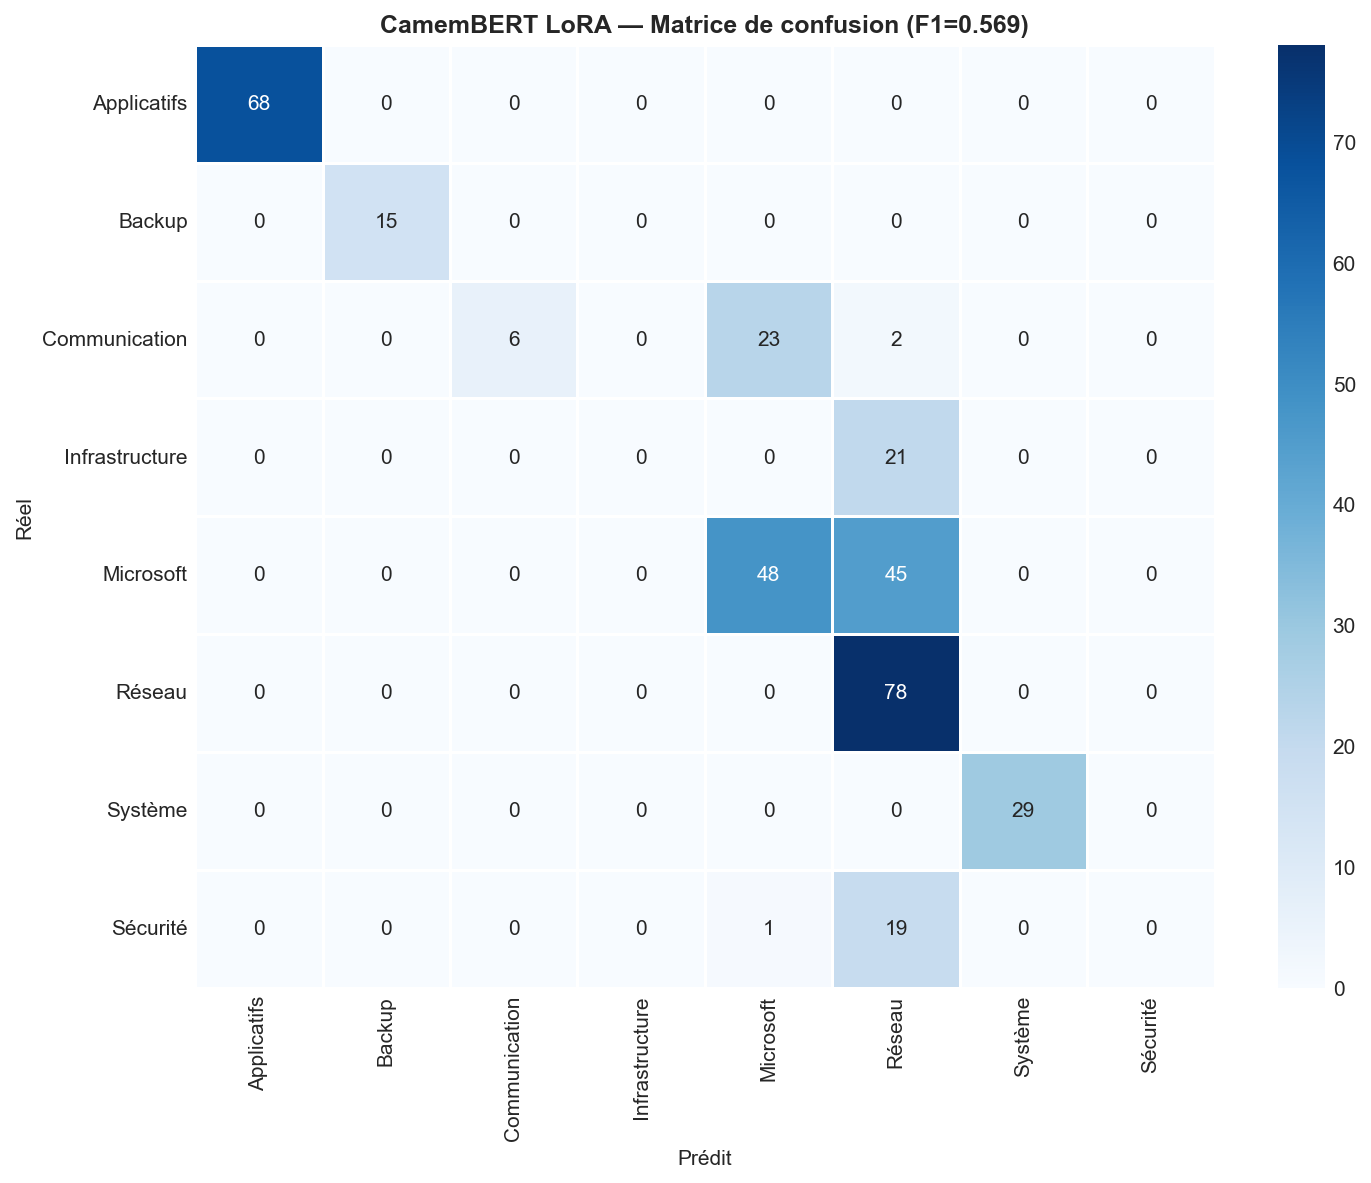
\includegraphics[width=0.92\textwidth]{ch04_confusion_camembert.png}
\caption{Matrice de confusion de CamemBERT adapté par LoRA}
\label{fig:camconf}
\end{figure}

Quatre catégories sont parfaitement traitées : \emph{Applicatifs}, \emph{Backup}, \emph{Réseau} et
\emph{Système}. \emph{Backup} est la surprise : la baseline y échouait totalement et les règles ne
la rattrapaient pas davantage.

Les erreurs se concentrent sur un point unique : \emph{Réseau} agit comme un attracteur. La totalité
des 21 tickets \emph{Infrastructure} y est versée, ainsi que 19 des 20 tickets \emph{Sécurité} et 45
des 93 tickets \emph{Microsoft}. Quand le modèle rencontre un scénario dont il n'a pas
l'équivalent, il le rattache à la catégorie dont il a vu la plus grande variété de formulations à
l'entraînement.

Le décompte sur \emph{Microsoft} se lit encore plus précisément. Les 93 tickets de cette catégorie
se répartissent en deux types, \og Microsoft Teams ne se lance plus \fg{} pour 48 d'entre eux et
\og OneDrive ne synchronise pas les fichiers \fg{} pour les 45 autres. Or le modèle classe
correctement 48 tickets et en verse 45 dans \emph{Réseau} : il traite le premier type sans aucune
erreur et le second sans aucune réussite. La décision se joue donc scénario par scénario : le sort
d'un ticket est celui de son type. Ce que le chapitre~3 avait établi sur les données se vérifie ici
sur les prédictions.

Préfixer chaque ticket de son type de demande et de sa priorité simplifiés, variables construites
au chapitre~3, fait passer le F1-macro de 0,5325 à 0,5685, soit un gain de 0,036. Ce préfixe donne
au modèle un signal que le texte libre ne porte pas toujours.

\section{Comparaison et analyse}

\subsection{Tableau d'ensemble}

La figure~\ref{fig:bench4} rassemble les sept approches sous le protocole unique de la
section~\ref{sec:protocole}.

\begin{figure}[!htbp]
\centering
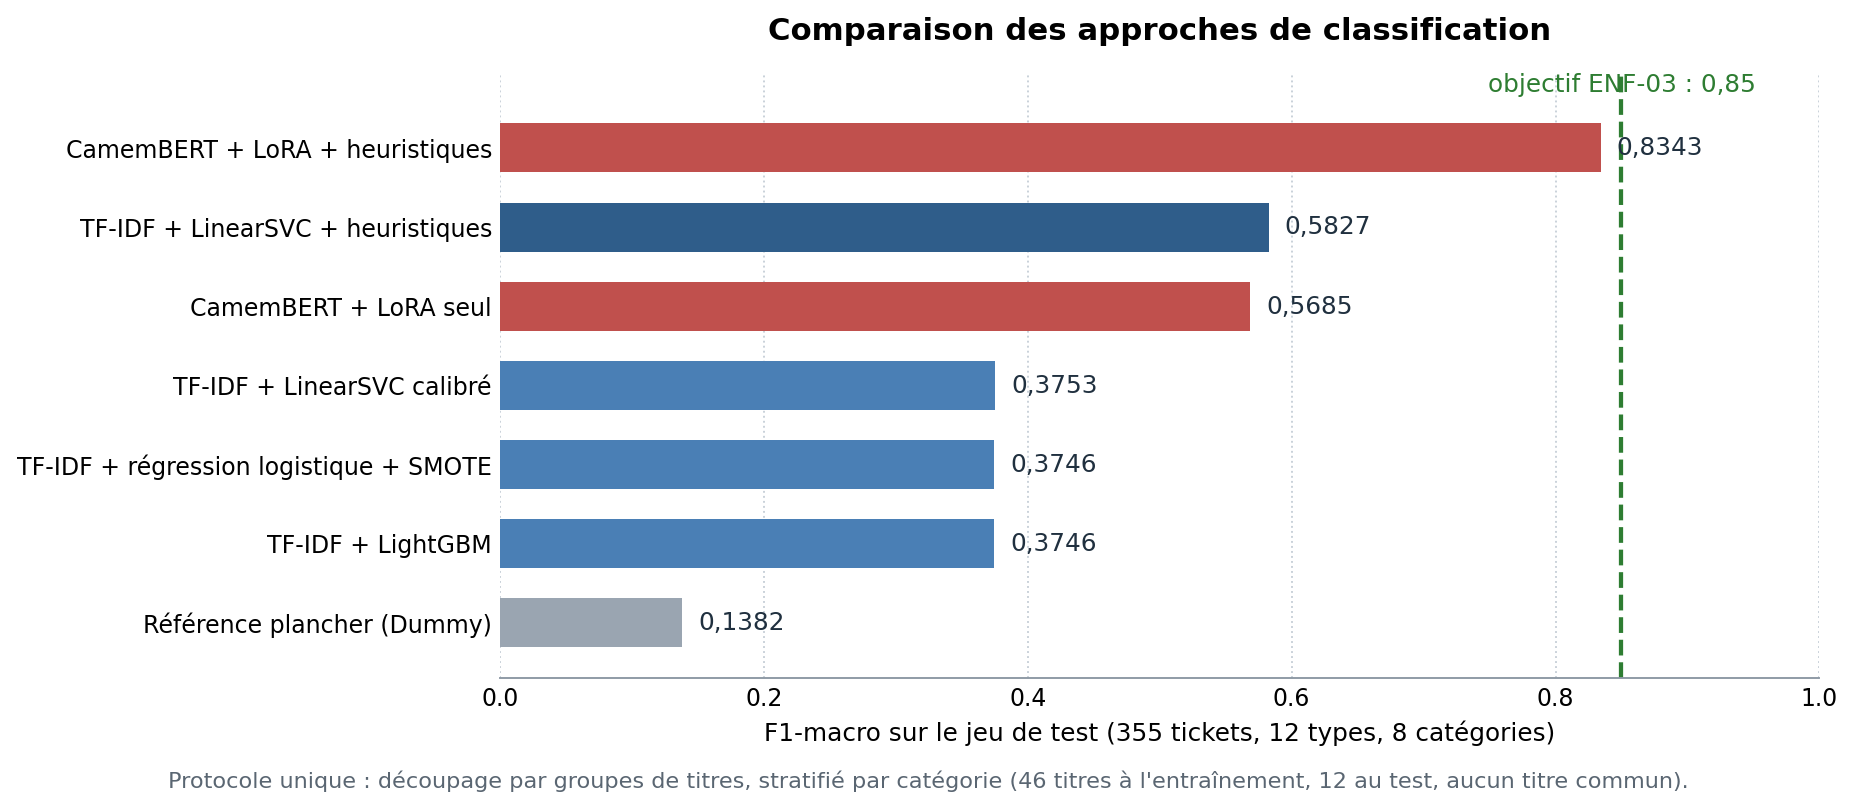
\includegraphics[width=\textwidth]{ch04_benchmark.png}
\caption{F1-macro des approches comparées, jeu de test de 355 tickets}
\label{fig:bench4}
\end{figure}

Quatre paliers se lisent sur ce graphique. Le hasard occupe le premier à 0,138. Les modèles
purement lexicaux forment le deuxième autour de 0,375, quelle que soit leur famille. Le troisième,
autour de 0,58, réunit l'approche par règles et le transformer seul. Le quatrième n'est occupé que
par leur combinaison, à 0,8343.

\subsection{La combinaison qui manquait}
\label{sec:combinaison}

La comparaison telle qu'elle vient d'être conduite oppose une chaîne lexicale complétée par des
règles à un transformer qui n'en reçoit aucune. Les deux systèmes ne sont donc pas dans la même
configuration, et l'écart mesuré entre eux ne dit rien de leurs mérites respectifs.

Les règles ne dépendent pourtant d'aucun modèle. Elles lisent le texte brut du ticket et reçoivent
une catégorie prédite accompagnée d'un score de confiance, sans se soucier de leur provenance. Rien
n'empêchait donc de les appliquer aux sorties de CamemBERT. Le tableau~\ref{tab:croise} donne les
quatre combinaisons.

\begin{table}[!htbp]
\centering
\styletableau
\caption{Les deux modèles, avec et sans les règles métier}
\label{tab:croise}
\begin{tabular}{|Bp{4.0cm}|Cp{2.8cm}|Cp{2.8cm}|Cp{2.6cm}|}
\hline
\rowcolor{enteteTab}
& \textbf{TF-IDF} & \textbf{CamemBERT} & \textbf{Écart} \\
\hline
Sans les règles & 0,3753 & 0,5685 & +0,1932 \\
\hline
Avec les règles & 0,5827 & \textbf{0,8343} & +0,2516 \\
\hline
Apport des règles & +0,2074 & +0,2658 & \\
\hline
\end{tabular}
\end{table}

Le tableau se lit dans les deux sens et donne deux résultats.

Dans les deux configurations, CamemBERT devance la chaîne lexicale, de 0,19 sans les règles et de
0,25 avec. L'hypothèse H1 du cahier des charges, selon laquelle un transformer francophone adapté
surpasse la baseline, est donc vérifiée. La lecture inverse, celle d'une égalité entre les deux
approches, provenait uniquement de la comparaison asymétrique.

Les règles profitent davantage au transformer qu'à la chaîne lexicale, +0,266 contre +0,207. Les
deux composants ne corrigent pas les mêmes erreurs. CamemBERT traite seul \emph{Backup} et
\emph{Système} à 1,00, là où la chaîne lexicale les abandonne ; les règles récupèrent
\emph{Infrastructure} et \emph{Sécurité}, que les deux modèles laissent à zéro. Leur combinaison
additionne deux couvertures complémentaires plutôt que de renforcer la même.

\subsection{Audit des règles métier}
\label{sec:audit}

Une vérification conduite en fin de sprint a révisé ces chiffres à la baisse, et la démarche mérite
d'être rapportée.

Les règles avaient été enrichies au fil des expériences. En reprenant leur historique, nous avons
constaté qu'un commentaire du code justifiait l'ajout d'un mot-clé par un titre appartenant au jeu
de test. Nous avons alors confronté chaque mot-clé au jeu d'entraînement. Quatre d'entre eux, réunis
au tableau~\ref{tab:audit}, n'y figuraient dans aucun ticket et ne se déclenchaient que sur des
tickets de test.

\begin{table}[!htbp]
\centering
\styletableau
\caption{Mots-clés retirés à l'issue de l'audit}
\label{tab:audit}
\begin{tabular}{|Bp{4.0cm}|Lp{3.4cm}|Cp{2.6cm}|Cp{2.6cm}|}
\hline
\rowcolor{enteteTab}
\textbf{Mot-clé} & \textbf{Catégorie forcée} & \textbf{Tickets d'entraînement} &
\textbf{Tickets de test} \\
\hline
\texttt{onedrive} & Microsoft & 0 & 45 \\
\hline
\texttt{san} & Infrastructure & 0 & 21 \\
\hline
\texttt{ids} & Sécurité & 0 & 12 \\
\hline
\texttt{acces non autorisé} & Sécurité & 0 & redondant \\
\hline
\end{tabular}
\end{table}

Un mot-clé introduit après avoir observé une erreur sur le jeu de test ajuste le système aux
données qui servent à le juger. Le score cesse alors de mesurer la généralisation et mesure la
mémorisation. Nous avons donc retiré ces quatre termes et remesuré l'ensemble des configurations.

L'effet est considérable. Le F1-macro de CamemBERT accompagné des règles passe de 0,9499 à 0,8343,
et celui de la chaîne lexicale de 0,7513 à 0,5827. La part non généralisable atteignait donc 0,116
d'un côté et 0,169 de l'autre. Tous les chiffres de ce chapitre sont ceux mesurés après retrait.

Ces quatre termes désignent pourtant des technologies dont la catégorie ne prête pas à discussion :
OneDrive est un produit Microsoft, un IDS un équipement de détection d'intrusion, un SAN une baie
de stockage. Le défaut ne tient pas à leur contenu mais au moment de leur introduction. Ils
pourraient être réintroduits si le service support les validait par écrit comme référentiel métier,
établi sans consultation des résultats de test. Cette validation n'a pas été obtenue dans le temps
du projet.

La règle de conduite retenue pour la suite figure désormais en tête du module de règles : un
mot-clé n'y est admis que s'il est attesté dans le jeu d'entraînement, ou s'il reste sans effet sur
le jeu de test.

\subsection{Ce qui sépare encore de l'objectif}
\label{sec:pourquoi}

Il manque 0,016 de F1-macro pour atteindre l'exigence ENF-03. Le détail par catégorie situe
précisément ce qui manque.

Six catégories sur huit dépassent 0,74 et quatre atteignent 1,00. La plus faible est
\emph{Microsoft}, à 0,4463, dont les 93 tickets de test se répartissent en deux scénarios : le
modèle traite le premier sans erreur et manque le second, faute du terme discriminant que l'audit a
écarté. Sa précision reste élevée, 0,96, mais son rappel tombe à 0,29.

Comme le F1-macro accorde un huitième du total à chaque catégorie, il suffirait que
\emph{Microsoft} passe de 0,4463 à 0,5719 pour franchir la barre des 0,85. Aucune autre catégorie
n'aurait besoin de bouger.

La limite de fond reste celle qu'a posée le chapitre~3. Le corpus contient 1\,800 tickets pour
58 scénarios distincts, dont 46 servent à l'entraînement. Ces 46 situations, répétées une trentaine
de fois chacune, sont tout ce dont dispose un modèle de langue conçu pour vivre de la diversité.
Ce qu'il faut ajouter au corpus se compte en scénarios, pas en tickets : multiplier les instances
d'un scénario déjà présent revient à recopier ce que le modèle sait déjà. Le chapitre~7 revient sur
ce point à propos de la boucle d'amélioration continue, qui vise précisément à faire entrer de
nouveaux scénarios au fil de l'exploitation.

\subsection{Le modèle retenu pour la production}
\label{sec:production}

Le système servi est le LinearSVC calibré accompagné des règles métier. Ce choix a été arrêté au
moment où les deux approches paraissaient équivalentes, et il reposait sur trois arguments
étrangers à la performance.

L'inférence de CamemBERT exige de charger 110 millions de paramètres, là où la chaîne TF-IDF tient
dans un fichier de 326\,ko. L'exigence ENF-01 fixe la latence de prédiction à 300\,ms au
quatre-vingt-quinzième centile, et le chapitre~7 montrera qu'elle n'est déjà pas tenue avec la
chaîne légère : lui substituer un transformer aggraverait un écart existant. Enfin, une décision
produite par des règles nommées s'explique au consultant, et le chapitre~1 a placé ce système en
position d'assistant.

La comparaison à configuration égale déplace cet arbitrage. Un écart de 0,25 de F1-macro ne se
compense pas par la légèreté d'un artefact, d'autant que les deux systèmes partagent la même couche
de règles et donc la même explicabilité sur les décisions qu'elle produit. La mise en service de
CamemBERT suppose de traiter d'abord la latence, par exemple en réservant le transformer aux
tickets dont la chaîne lexicale n'est pas sûre. Nous la portons aux perspectives plutôt que de
l'engager en fin de projet.

L'adaptateur reste versionné dans le dépôt et la porte de promotion décrite au chapitre~7 accepte
un modèle de cette nature, à condition qu'il soit évalué sur le même jeu de test gelé.

Nous conservons l'adaptateur CamemBERT dans le dépôt. Il documente la comparaison et resterait
mobilisable si le corpus gagnait en diversité.

Le pipeline réentraîne le modèle de production, donc sous le découpage non stratifié.
Ses chiffres, rapportés au tableau~\ref{tab:prod}, ne sont pas comparables à ceux qui précèdent.

\begin{table}[!htbp]
\centering
\styletableau
\caption{Modèle de production, mesuré sous le protocole du pipeline}
\label{tab:prod}
\begin{tabular}{|Bp{6.2cm}|Cp{2.6cm}|Lp{4.4cm}|}
\hline
\rowcolor{enteteTab}
\textbf{Indicateur} & \textbf{Valeur} & \textbf{Portée} \\
\hline
F1-macro, modèle seul & 0,2708 & 8 catégories \\
\hline
F1-macro avec les règles & 0,5829 & 8 catégories, dont 3 sans exemple \\
\hline
F1-macro sur les catégories évaluables & 0,6995 & 5 catégories ayant du support \\
\hline
Exactitude & 0,8202 & 356 tickets \\
\hline
Précision macro & 0,5868 & 5 catégories \\
\hline
Rappel macro & 0,6099 & 5 catégories \\
\hline
Part des tickets corrigés par une règle & 37,4\,\% & 356 tickets \\
\hline
\end{tabular}
\end{table}

Les trois catégories absentes du jeu de test expliquent seules l'écart entre 0,5829 et 0,6995 :
leur F1 vaut zéro parce qu'aucun ticket ne les représente, non parce que le modèle les manque. Nous
rapportons les deux valeurs ; la seconde sert de métrique de décision au mécanisme de promotion
décrit au chapitre~7. Aucune des deux n'est comparable au 0,5827 du protocole stratifié.

Le rappel sur \emph{Sécurité} tombe à zéro sous ce protocole, pour une exigence ENF-04 fixée à
0,70. Les trois scénarios de sécurité tirés au test relèvent tous de l'intrusion détectée, et le
terme qui les caractérisait a été écarté par l'audit. Le même système atteint un rappel de 0,40 sur
cette catégorie sous le protocole stratifié, où d'autres scénarios sont tirés. Cet écart de zéro à
0,40 pour un système inchangé illustre ce que le chapitre~3 annonçait : sur douze scénarios de
test, une mesure par catégorie se déplace par paliers entiers.

\subsection{Calibration de la confiance et routage}
\label{sec:calibration}

Le système renvoie un score de confiance destiné à décider quels tickets peuvent être routés
automatiquement et lesquels demandent une revue humaine. Encore faut-il que ce score ordonne
correctement la fiabilité. Le tableau~\ref{tab:calib} confronte les tranches de confiance à la
précision réellement observée dans chacune.

\begin{table}[!htbp]
\centering
\styletableau
\caption{Précision observée par tranche de confiance, protocole des expériences}
\label{tab:calib}
\begin{tabular}{|Bp{3.0cm}|Cp{2.4cm}|Cp{2.2cm}|Cp{2.6cm}|}
\hline
\rowcolor{enteteTab}
\textbf{Tranche} & \textbf{Tickets} & \textbf{Part} & \textbf{Précision} \\
\hline
Sous 40\,\% & 42 & 11,8\,\% & 0,0\,\% \\
\hline
40 à 60\,\% & 121 & 34,1\,\% & 33,9\,\% \\
\hline
60 à 80\,\% & 110 & 31,0\,\% & 89,1\,\% \\
\hline
Au-dessus de 80\,\% & 82 & 23,1\,\% & 81,7\,\% \\
\hline
\end{tabular}
\end{table}

Le score sépare correctement les deux extrémités : sous 40\,\%, aucune prédiction n'est juste ;
au-delà de 60\,\%, plus de quatre sur cinq le sont. La distribution de la
figure~\ref{fig:confiance} montre cette séparation sur le modèle CamemBERT.

\begin{figure}[!htbp]
\centering
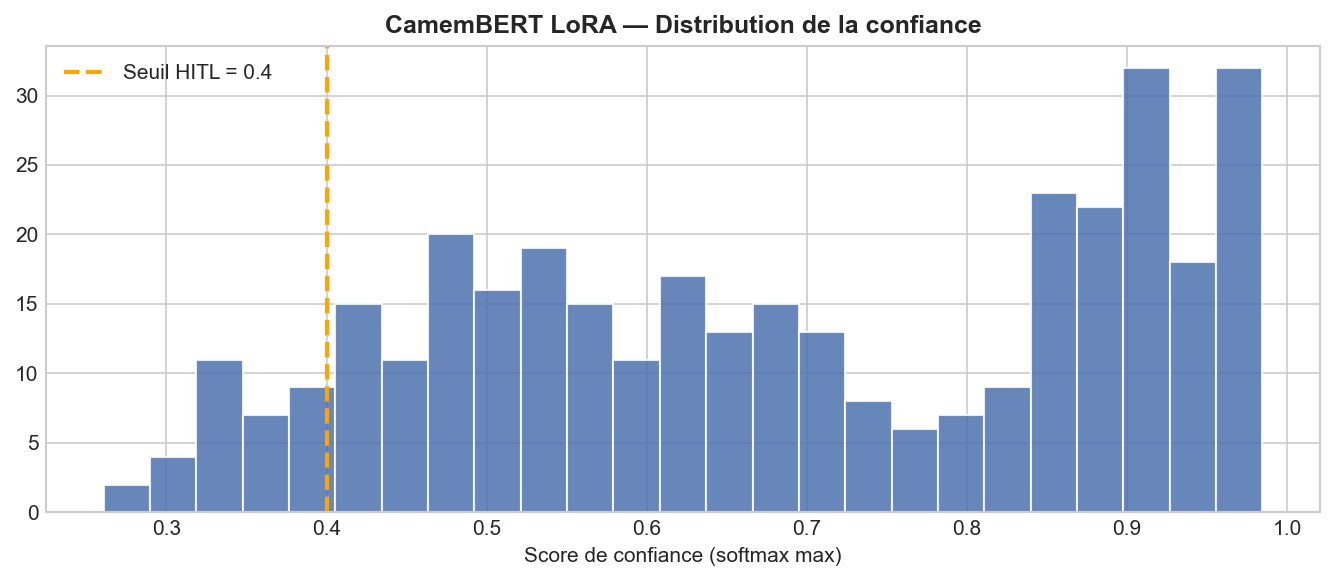
\includegraphics[width=0.92\textwidth]{ch04_confiance.png}
\caption{Distribution des scores de confiance et seuil de routage}
\label{fig:confiance}
\end{figure}

Une anomalie subsiste néanmoins. La tranche 60 à 80\,\% est plus fiable, à 89,1\,\%, que la tranche
supérieure à 80\,\%, qui tombe à 81,7\,\%. Un score de confiance devrait être monotone : plus il est
élevé, plus la prédiction devrait être sûre. Il ne l'est pas ici. Le score renseigne donc sur
l'ordre de grandeur de la fiabilité, sans permettre de distinguer finement deux prédictions toutes
deux assurées. C'est la réserve portée à l'objectif~6.

Nous avions d'abord fixé le seuil de routage à 0,40, valeur qui envoie 88,2\,\% des tickets en
traitement automatique pour une précision de 65,8\,\%. Un tel réglage laisse passer un tiers
d'erreurs sans relecture, ce qui contredit le principe de maintien de la décision humaine posé en
introduction du mémoire. Nous l'avons relevé à 0,60 dans la configuration de production. Les
métadonnées du modèle annoncent pour ce nouveau seuil environ 70\,\% de routage automatique et
85\,\% de précision ; il s'agit d'une estimation, que le jeu de test n'a pas servi à vérifier.

\section{Bilan du sprint}

Le sprint livre un protocole d'évaluation explicite, sept approches comparées sous ce protocole, un
module de règles métier audité, un adaptateur CamemBERT entraîné sous contrainte matérielle, et le
modèle servi en production avec son seuil de routage.

L'exigence ENF-03 visait 0,85 et la meilleure combinaison atteint 0,8343 sous le protocole
stratifié. L'écart de 0,016 tient à une seule catégorie, \emph{Microsoft}, dont le terme
discriminant a été écarté faute de support à l'entraînement.

L'exigence ENF-04 visait un rappel d'au moins 0,70 sur \emph{Sécurité}, et elle n'est atteinte dans
aucune configuration. Le meilleur rappel mesuré est 0,60, obtenu par CamemBERT accompagné des
règles sur le protocole stratifié ; la chaîne lexicale plafonne à 0,40 sur le même jeu et à zéro
sous le protocole du pipeline. La précision, elle, vaut 1,00 dans les deux cas : chaque incident de
sécurité annoncé en est bien un, mais quatre sur dix échappent au système dans le meilleur des cas.
Nous reportons ces deux écarts au registre des risques du projet.

Le sprint livre aussi un résultat de méthode. L'audit des règles a retiré quatre mots-clés
introduits en observant le jeu de test et a fait baisser le meilleur score de 0,9499 à 0,8343. Un
projet qui ne mène pas cette vérification publie des chiffres qu'il croit sincères. Nous
considérons ce retrait comme un acquis du sprint au même titre que les modèles entraînés.

Le sprint établit enfin un diagnostic qui oriente la suite. Le plafond rencontré est celui des
46 scénarios distincts disponibles à l'entraînement. Deux conséquences en découlent pour le reste
du mémoire. Le chapitre~5 met la redondance du corpus à profit : un moteur de recherche par
similarité tire parti de ce qui embarrasse un classifieur. Le chapitre~7 construit le mécanisme qui
permettra au corpus de gagner des scénarios au fil de l'exploitation.

\section*{Conclusion}
\addcontentsline{toc}{section}{Conclusion}

Trois approches ont été éprouvées sous un protocole unique, qui couvre les huit catégories. La
vectorisation classique atteint 0,3753 et ignore la moitié du référentiel. Lui adjoindre les règles
métier porte le résultat à 0,5827 : les catégories abandonnées reviennent. CamemBERT adapté par
LoRA atteint 0,5685 sans aucune règle.

Le résultat décisif vient de leur combinaison, que la comparaison initiale n'avait pas éprouvée.
Les règles ne dépendent d'aucun modèle : elles lisent le texte brut et corrigent une catégorie
prédite, quelle qu'en soit l'origine. Appliquées aux sorties du transformer, elles portent le
F1-macro à \textbf{0,8343}, à 0,016 de l'objectif. CamemBERT devance la chaîne lexicale dans les
deux configurations, de 0,19 sans les règles et de 0,25 avec, ce qui vérifie l'hypothèse H1 du
cahier des charges.

Ce chiffre est celui qui subsiste après l'audit des règles. Quatre mots-clés absents du jeu
d'entraînement et actifs sur le seul jeu de test ont été retirés, ce qui a ramené le meilleur score
de 0,9499 à 0,8343. La différence mesurait ce que le système avait mémorisé plutôt qu'appris.

Le modèle mis en service reste la chaîne TF-IDF complétée par les règles, choisie pour sa latence
et sa légèreté à un moment où les deux approches paraissaient équivalentes. L'écart désormais
mesuré invite à rouvrir cet arbitrage, ce que la conclusion générale porte aux perspectives. Le
score de confiance sépare utilement les prédictions fiables des autres sans être strictement
monotone, ce qui justifie de conserver la revue humaine sur les cas peu assurés.

Le chapitre~5 construit le second volet de la solution : un moteur de recherche qui retrouve dans
l'historique les résolutions comparables, et pour lequel la redondance du corpus devient un atout.
